\chapter{细胞与病毒的基因组}\label{ch:b1:genomes}

两米长的 \omterm{def:b1:nucleic-acids:chain}{DNA} 被折叠进直径为六微米的\omterm{def:b1:eukaryotic-cell:nucleus}{细胞核}中，
并且折叠得使两万个\omterm{def:b1:genomes:gene}{基因}中的任一个都能被找到并读取，
只需几分钟。细菌把一毫米半长的 \omterm{def:b1:nucleic-acids:chain}{DNA} 折叠进
一个短一千倍的\omterm{def:b1:cell-unit-of-life:cell}{细胞}中，每二十分钟复制一次。\omterm{def:b1:genomes:virus}{病毒}
在\omterm{def:b1:proteins:peptide}{蛋白质}外壳中携带几千个字母，并借助
一个并不属于它的\omterm{def:b1:cell-unit-of-life:cell}{细胞}来读取。本章描述\emph{\omterm{def:b1:genomes:genome}{基因组}}——
即一个\omterm{def:b1:organism-environment:organism}{生物体}的全部 \omterm{def:b1:nucleic-acids:chain}{DNA}——，作为一种物理对象，考察
细菌、\omterm{def:b1:cell-unit-of-life:prokeuk}{真核细胞}、\omterm{def:b1:eukaryotic-cell:organelle}{细胞器}和\omterm{def:b1:genomes:virus}{病毒}的 \omterm{def:b1:nucleic-acids:chain}{DNA} 如何\omterm{def:b1:body-plans-tissues:tissue}{组织}，
它除\omterm{def:b1:genomes:gene}{基因}外还含有什么，以及 \omterm{def:b1:nucleic-acids:chain}{DNA} 的含量为何
对携带它的\omterm{def:b1:organism-environment:organism}{生物体}几乎说明不了问题。

\section{细菌的基因组}

\begin{definition}[基因组、染色体、拟核]\label{def:b1:genomes:genome}
一个\omterm{def:b1:cell-unit-of-life:cell}{细胞}的\emph{基因组}\index{基因组}是其全部 \omterm{def:b1:nucleic-acids:chain}{DNA} 的总和：
即它能够制造的每种\omterm{def:b1:proteins:peptide}{蛋白质}和 \omterm{def:b1:nucleic-acids:chain}{RNA} 的信息，以及
控制它们何时被制造的序列。\emph{染色体}\index{染色体}是
一条 \omterm{def:b1:nucleic-acids:chain}{DNA} 分子连同\omterm{def:b1:body-plans-tissues:tissue}{组织}它的\omterm{def:b1:proteins:peptide}{蛋白质}。一个细菌通常只有一条，
呈环状，含一百万至一千万个\omterm{thm:b1:nucleic-acids:helix}{碱基对}
（\emph{E. coli}：$\num{4.6e6}$，\qty{1.5}{mm}长），折叠成一个
\omterm{def:b1:cell-unit-of-life:cell}{细胞质}中的一个区域，即\emph{拟核}\index{拟核}，外面没有
膜包围。除染色体外，许多细菌还携带
\emph{质粒}\index{质粒}：几千至几十万个\omterm{thm:b1:nucleic-acids:helix}{碱基对}的小环，
每个\omterm{def:b1:cell-unit-of-life:cell}{细胞}含一至数百个拷贝，可独立复制，
并携带非必需\omterm{def:b1:genomes:gene}{基因}——如抗生素抗性、毒素，
以及将自身转移到另一\omterm{def:b1:cell-unit-of-life:cell}{细胞}的机制。
\end{definition}

\begin{proposition}[细菌如何折叠其染色体]\label{prop:b1:genomes:supercoiling}
\index{超螺旋}
两端不能转动的环状 \omterm{def:b1:nucleic-acids:chain}{DNA} 可像橡皮筋那样被扭转，此即
\emph{超螺旋}。称为\emph{拓扑异构酶}的酶能切断、
让链穿过后再封合，以增减扭转圈数；\emph{促旋酶}利用
\omterm{def:b1:water-small-molecules:atp}{ATP} 引入负超螺旋，使螺旋欠旋，
从而既更紧凑又更易于打开。\emph{E. coli}的\omterm{def:b1:genomes:genome}{染色体}
被\omterm{def:b1:body-plans-tissues:tissue}{组织}为约五十个环，
每个环独立超螺旋并锚定于\omterm{def:b1:proteins:peptide}{蛋白质}核心，使
\qty{1.5}{mm}长的\omterm{def:b1:genomes:genome}{染色体}占据约一微米的\omterm{def:b1:genomes:genome}{拟核}——
压缩约一千倍——而任一环都可单独展开，以供读取
或复制，而不影响其余部分。小型碱性\omterm{def:b1:proteins:peptide}{蛋白质}
（类\omterm{def:b1:genomes:nucleosome}{组蛋白}，但与\omterm{def:b1:genomes:nucleosome}{组蛋白}并无亲缘关系）使 \omterm{def:b1:nucleic-acids:chain}{DNA} 弯曲、桥接
贯穿整条 \omterm{def:b1:nucleic-acids:chain}{DNA}。
\end{proposition}

\begin{omfigure}
\begin{tikzpicture}[font=\footnotesize, line cap=round]
  % relaxed circle
  \draw[very thick, omDef] (0,0) circle (1.1);
  \node[anchor=north, align=center] at (0,-1.35) {松弛环状 \\ （每圈 10.5 bp）};
  % supercoiled: figure-eight / plectoneme
  \draw[very thick, omDef, domain=0:360, samples=240, smooth, variable=\t] plot ({4.3+1.05*cos(\t)}, {0.32*sin(4*\t)});
  \node[anchor=north, align=center] at (4.3,-1.35) {负超螺旋：\\ 欠旋，紧凑};
  \draw[->, thick] (1.35,0.15) -- (3.1,0.15) node[midway, above, align=center] {促旋酶（ATP）};
  \draw[->, thick] (3.1,-0.25) -- (1.35,-0.25) node[midway, below, align=center] {拓扑异构酶 I};
  % looped nucleoid
  \fill[omProp!40] (8.7,0) circle (0.35);
  \foreach \a in {0,45,...,315} {
    \draw[very thick, omDef] (8.7,0) .. controls ({8.7+1.6*cos(\a-20)},{1.6*sin(\a-20)}) and ({8.7+1.6*cos(\a+20)},{1.6*sin(\a+20)}) .. (8.7,0);
  }
  \node[anchor=north, align=center] at (8.7,-1.35) {拟核：约五十个 \\ 超螺旋环，附着于蛋白质核心};
\end{tikzpicture}

{\small 环状\omterm{def:b1:genomes:genome}{染色体}松弛、超螺旋，并\omterm{def:b1:body-plans-tissues:tissue}{组织}成
环。超螺旋使分子压缩，并储存有助于打开它的能量；
环结构则使一次只需展开一个区域。}
\end{omfigure}

\begin{example}[紧密排列的基因组]\label{ex:b1:genomes:dense}
\emph{E. coli}\omterm{def:b1:genomes:genome}{染色体}（\qty{4.6}{Mb}）中，\qty{88}{\%}
用于编码\omterm{def:b1:proteins:peptide}{蛋白质}：约 \num{4300} 个\omterm{def:b1:genomes:gene}{基因}，每个约 \num{1000} 个\omterm{thm:b1:nucleic-acids:helix}{碱基对}，
首尾紧密排列，相邻之间相隔约一百个\omterm{thm:b1:nucleic-acids:helix}{碱基对}，许多
聚集为共同转录的\emph{操纵子}（见\cref{ch:b1:expression-control}）。
一个 \qty{5}{kb} 的\omterm{def:b1:genomes:genome}{质粒}可携带三个\omterm{def:b1:genomes:gene}{基因}，并以
五十个拷贝存在；它所携带的抗性\omterm{def:b1:genomes:gene}{基因}可在医院病房的
细菌之间数周内即可借接合扩散，速度快于任何突变
所能产生的速度。
\end{example}

\section{真核基因组：染色质}

\begin{definition}[核小体、染色质]\label{def:b1:genomes:nucleosome}
\index{核小体}\index{组蛋白}\index{染色质}
在\omterm{def:b1:cell-unit-of-life:prokeuk}{真核细胞}核中，\omterm{def:b1:nucleic-acids:chain}{DNA} 缠绕在\omterm{def:b1:proteins:peptide}{蛋白质}上：\qty{147}{} 个\omterm{thm:b1:nucleic-acids:helix}{碱基对}
缠绕由八个\emph{组蛋白}组成的八聚体 1.7 圈，
（每种两个：H2A、H2B、H3、H4，均为富含赖氨酸和
精氨酸的小蛋白，可中和磷酸基团），形成一个
直径为 \qty{11}{nm} 的\emph{核小体}\index{核小体}，
核小体依次排列，每隔约 \qty{200}{} 个\omterm{thm:b1:nucleic-acids:helix}{碱基对}一个，像串在线上的珠子，
另有第五种组蛋白 H1 封住每颗珠子。这
\emph{染色质}进一步折叠：形成直径 \qty{30}{nm} 的纤维，
再形成数万个\omterm{thm:b1:nucleic-acids:helix}{碱基对}的环，锚定在\omterm{def:b1:proteins:peptide}{蛋白质}支架上，
并且在分裂时，形成致密的棒状中期\omterm{def:b1:genomes:genome}{染色体}，
长度比裸露 \omterm{def:b1:nucleic-acids:chain}{DNA} 缩短一万倍。
\emph{常染色质}是间期中松散、富含\omterm{def:b1:genomes:gene}{基因}、正在转录的形式；
\emph{异染色质}则是致密、\omterm{def:b1:genomes:gene}{基因}稀少、保持紧缩的形式
（位于\omterm{def:b1:genomes:karyotype}{着丝粒}周围、末端，以及失活的
X \omterm{def:b1:genomes:genome}{染色体}上）。
\end{definition}

\begin{omfigure}
\begin{tikzpicture}[font=\footnotesize, >=Stealth, line cap=round]
  % level 1: double helix line
  \draw[very thick, omDef] (0,5.4) -- (3.2,5.4);
  \node[anchor=west, align=left] at (3.5,5.4) {双螺旋，\qty{2}{nm}};
  % level 2: beads on a string
  \draw[thick, omDef] (0,4.2) -- (3.2,4.2);
  \foreach \x in {0.4,1.2,2.0,2.8} { \fill[omProp!70] (\x,4.2) circle (0.22); \draw[thick, omDef] (\x,4.2) circle (0.3); }
  \node[anchor=west, align=left] at (3.5,4.2) {核小体，\qty{11}{nm}：\qty{147}{bp} 缠绕组蛋白八聚体，\\ 每 \qty{200}{bp} 一个——压缩 $\times 6$};
  % level 3: 30 nm fibre (zigzag stack)
  \foreach \i in {0,...,9} { \fill[omProp!70] (0.2+0.3*\i,{3.0+0.18*(-1)^\i}) circle (0.17); }
  \node[anchor=west, align=left] at (3.5,3.0) {\qty{30}{nm} 纤维：核小体堆叠——$\times 40$};
  % level 4: loops on scaffold
  \draw[very thick, gray] (0,1.5) -- (3.2,1.5);
  \foreach \x in {0.4,1.2,2.0,2.8} { \draw[thick, omProp!80!black] (\x,1.5) .. controls (\x-0.35,2.3) and (\x+0.35,2.3) .. (\x,1.5); }
  \node[anchor=west, align=left] at (3.5,1.8) {\qtyrange{50}{100}{kb} 环附着于支架，\qty{300}{nm}——$\times 1000$};
  % level 5: metaphase chromosome
  \draw[very thick, omThm, fill=omThm!30, rounded corners=4pt] (0.9,-0.3) rectangle (1.4,1.0);
  \draw[very thick, omThm, fill=omThm!30, rounded corners=4pt] (1.7,-0.3) rectangle (2.2,1.0);
  \fill[omThm!60!black] (1.55,0.45) ellipse (0.45 and 0.13);
  \node[anchor=west, align=left] at (3.5,0.35) {中期染色体，直径 \qty{1400}{nm}：$\times \num{10000}$\\ （\qty{8.5}{cm} 的 DNA 位于 \qty{10}{\micro m} 内）};
\end{tikzpicture}

{\small 真核生物 \omterm{def:b1:nucleic-acids:chain}{DNA} 的各级包装，从\omterm{thm:b1:nucleic-acids:helix}{双螺旋}到
中期\omterm{def:b1:genomes:genome}{染色体}。每一级都成倍提高压缩程度；
整体压缩可达一万倍。}
\end{omfigure}

\begin{omfigure}
\begin{minipage}[b]{0.46\linewidth}\centering
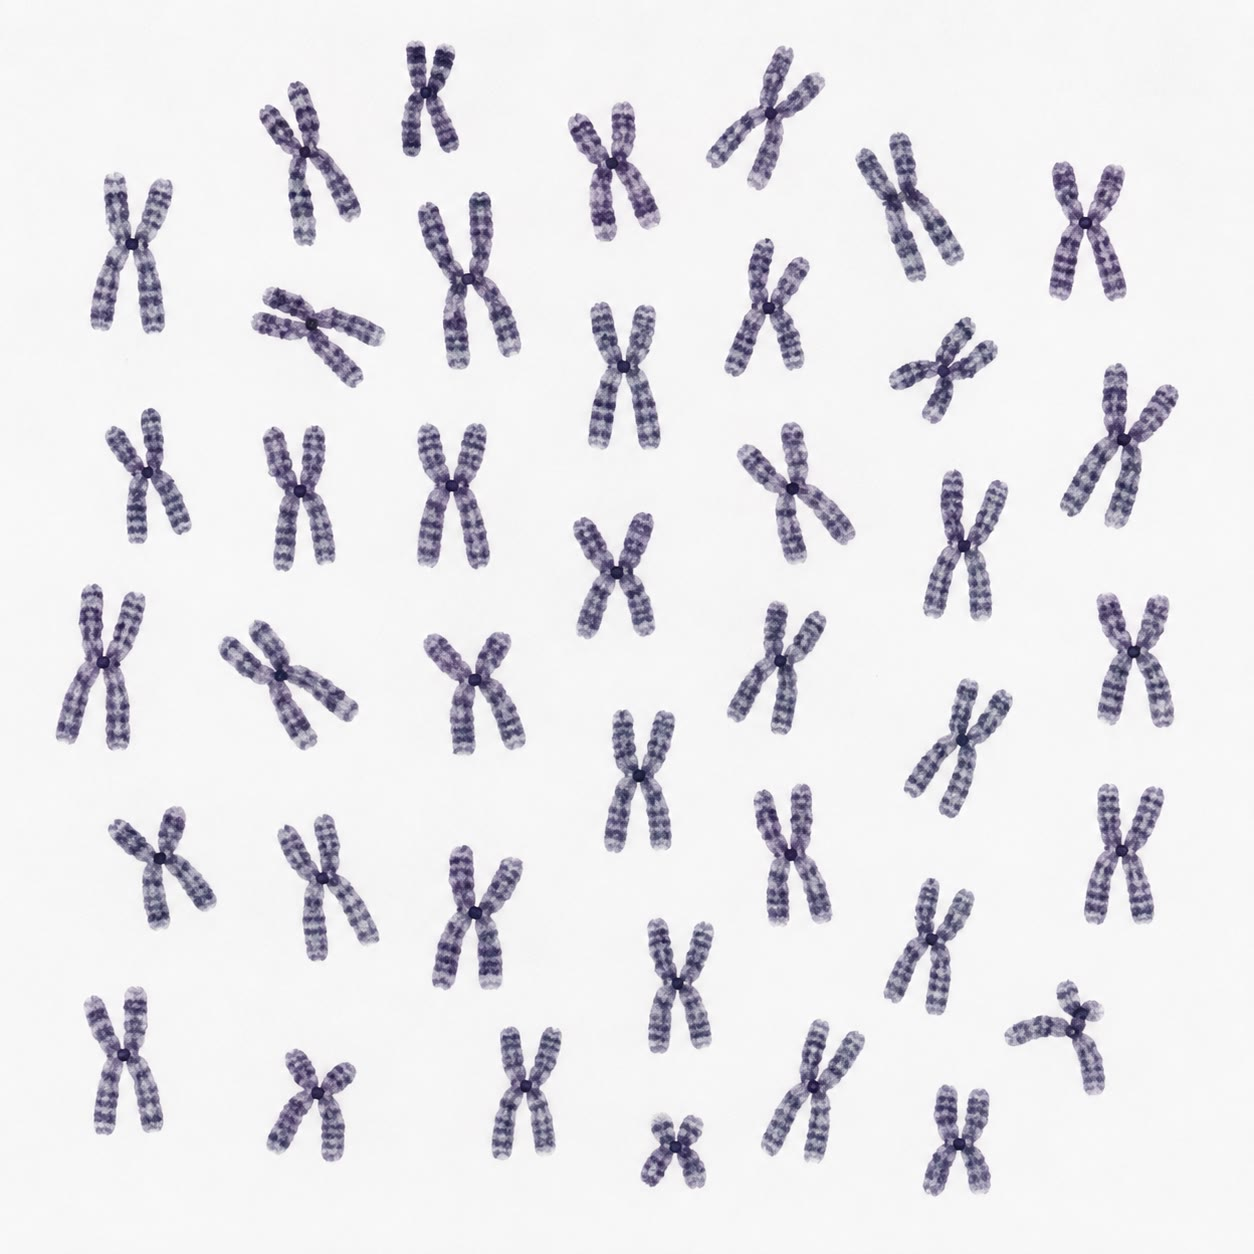
\includegraphics[width=0.94\linewidth]{images/book3/ai/b3-17-metaphase-spread.jpg}
\end{minipage}\hfill
\begin{minipage}[b]{0.5\linewidth}\centering
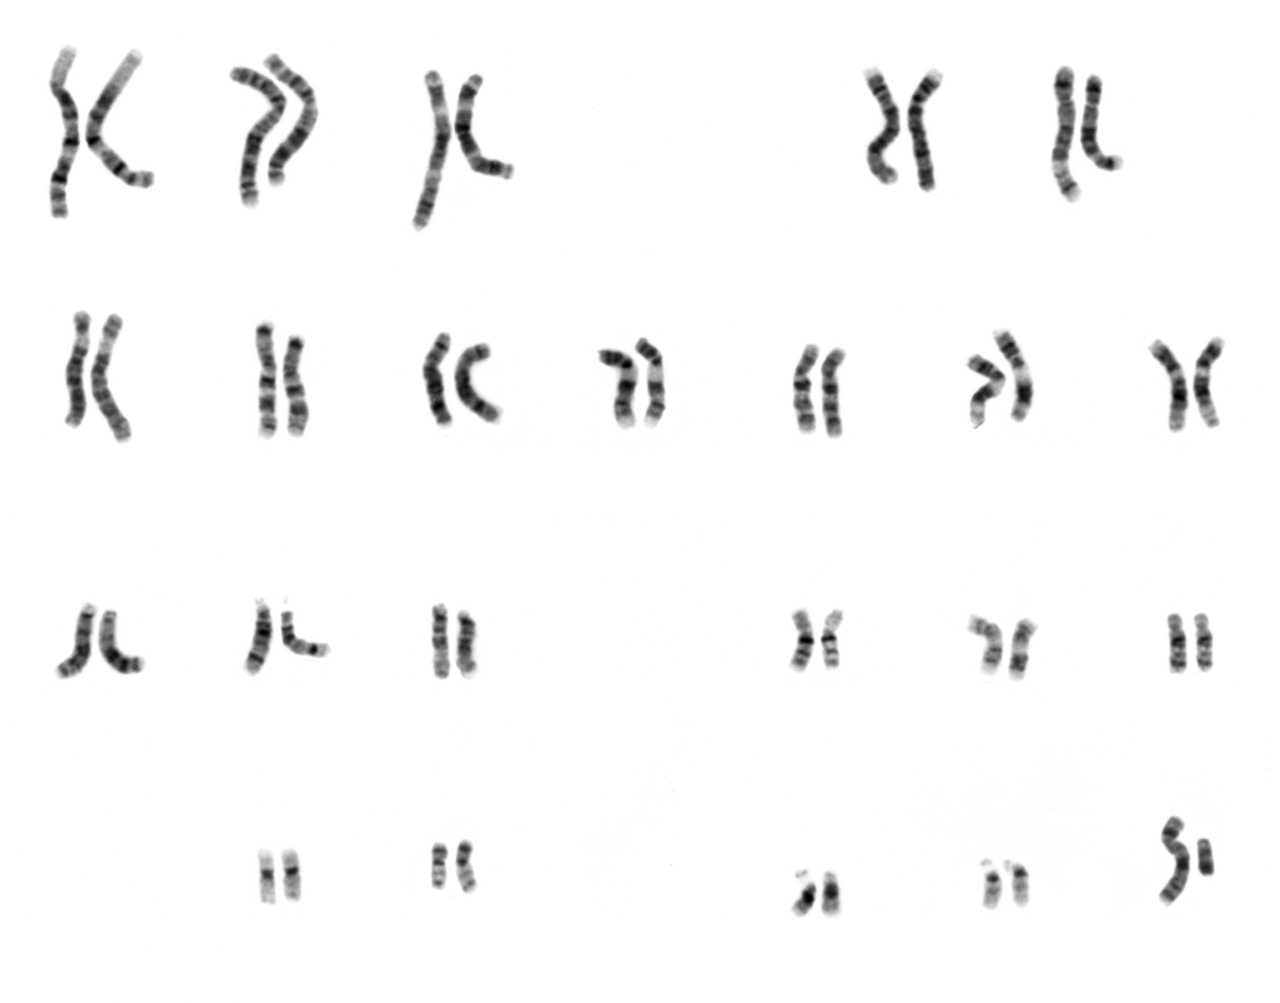
\includegraphics[width=0.96\linewidth]{images/book3/karyotype.png}
\end{minipage}

{\small 左图：取自中期阻滞\omterm{def:b1:cell-unit-of-life:cell}{细胞}的一个人类\omterm{def:b1:cell-unit-of-life:cell}{细胞}的\omterm{def:b1:genomes:genome}{染色体}铺片。
右图：同一批\omterm{def:b1:genomes:genome}{染色体}按大小和带型排列，
形成\omterm{def:b1:genomes:karyotype}{核型}图——22 对常\omterm{def:b1:genomes:genome}{染色体}和 XY，共 46 条。
\omterm{def:b1:genomes:karyotype}{核型}图：美国国家人类\omterm{def:b1:genomes:genome}{基因组}研究所，公有领域。}
\end{omfigure}

\begin{definition}[核型，着丝粒，端粒]\label{def:b1:genomes:karyotype}
\index{核型}\index{着丝粒}\index{端粒}
\emph{核型}是\omterm{def:b1:cell-unit-of-life:cell}{细胞}中全部\omterm{def:b1:genomes:genome}{染色体}的集合，按
大小和带型排列。人类有 23 对\omterm{def:b1:genomes:genome}{染色体}（22 对常\omterm{def:b1:genomes:genome}{染色体}加 XY 或
XX），共 $\num{6.4e9}$ 个\omterm{thm:b1:nucleic-acids:helix}{碱基对}，总长 \qty{2.2}{m}；最大的
\omterm{def:b1:genomes:genome}{染色体}含 \qty{250}{Mb}，最小的为 \qty{50}{}。每条线性
\omterm{def:b1:genomes:genome}{染色体}都带有一个\emph{着丝粒}，即复制后两条拷贝仍相连的
缢缩区域，纺锤体在此附着（
见\cref{ch:b1:replication-mitosis}）；两端各有一个\emph{端粒}，
是位于末端的重复序列，它们使\omterm{def:b1:genomes:genome}{染色体}不被误认为断裂的
\omterm{def:b1:nucleic-acids:chain}{DNA}，并防止每次复制时末端缩短。
\end{definition}

\begin{proposition}[基因组大小并不衡量复杂程度]\label{prop:b1:genomes:cvalue}
\index{C 值矛盾}
\begin{center}
\small
\begin{tabular}{lrr}
\hline
\omterm{def:b1:organism-environment:organism}{生物体} & \omterm{def:b1:genomes:genome}{基因组}（Mb） & 编码\omterm{def:b1:proteins:peptide}{蛋白质}的\omterm{def:b1:genomes:gene}{基因}数 \\
\hline
\emph{E. coli} & 4.6 & \num{4300} \\
酵母 & 12 & \num{6000} \\
果蝇 & 140 & \num{14000} \\
人 & 3200 & \num{20000} \\
玉米 & 2300 & \num{40000} \\
肺鱼 & \num{130000} & $\approx\num{20000}$ \\
\emph{Paris japonica}（一种百合） & \num{150000} & $\approx\num{30000}$ \\
\hline
\end{tabular}
\end{center}
真核生物的\omterm{def:b1:genomes:genome}{基因组}大小相差千倍，与\omterm{def:b1:genomes:gene}{基因}数目或\omterm{def:b1:organism-environment:organism}{生物体}的复杂程度无关
（即\emph{C 值矛盾}）：肺鱼所含的 \omterm{def:b1:nucleic-acids:chain}{DNA}
是人的四十倍，而\omterm{def:b1:genomes:gene}{基因}数并不更多。
差别不在于\omterm{def:b1:genomes:gene}{基因}，
而在于\omterm{def:b1:genomes:gene}{基因}之间的 \omterm{def:b1:nucleic-acids:chain}{DNA}。
\end{proposition}

\section{基因组的组成}

\begin{definition}[基因的结构]\label{def:b1:genomes:gene}
\index{基因}\index{外显子}\index{内含子}\index{启动子}
\emph{基因}是一段被转录为有功能的 \omterm{def:b1:nucleic-acids:chain}{RNA} 的 \omterm{def:b1:nucleic-acids:chain}{DNA} 序列，
通常是某种\omterm{def:b1:proteins:peptide}{蛋白质}的信使。真核生物编码\omterm{def:b1:proteins:peptide}{蛋白质}的
基因包括：\emph{启动子}，位于上游、转录在此起始并受
其调控的序列；\emph{外显子}，即保留在成熟信使中的部分；
\emph{内含子}，即被转录后再切除的部分；
（见\cref{ch:b1:gene-expression}）；信使两端不被翻译的
区域；以及终止子。人的基因平均长 \qty{27}{kb}，
八个外显子共 \qty{1.5}{kb}：一个典型基因的二十分之十九
是内含子。细菌基因
没有内含子。
\end{definition}

\begin{omfigure}
\begin{tikzpicture}[font=\footnotesize, >=Stealth, line cap=round]
  \draw[very thick, gray] (0,0) -- (12.6,0);
  \fill[omExo!50] (0.2,-0.18) rectangle (1.6,0.18); \node[anchor=north] at (0.9,-0.25) {启动子};
  \fill[omDef!70] (1.6,-0.25) rectangle (2.4,0.25);
  \fill[omDef!70] (4.6,-0.25) rectangle (5.6,0.25);
  \fill[omDef!70] (8.4,-0.25) rectangle (9.0,0.25);
  \fill[omDef!70] (10.9,-0.25) rectangle (12.0,0.25);
  \node[anchor=south, omDef!70!black] at (2.0,0.3) {外显子 1};
  \node[anchor=south, omDef!70!black] at (5.1,0.3) {外显子 2};
  \node[anchor=south, omDef!70!black] at (8.7,0.3) {外显子 3};
  \node[anchor=south, omDef!70!black] at (11.45,0.3) {外显子 4};
  \node[anchor=north] at (3.5,-0.3) {内含子 1};
  \node[anchor=north] at (7.0,-0.3) {内含子 2};
  \node[anchor=north] at (9.95,-0.3) {内含子 3};
  \draw[->, thick, omExo!70!black] (1.6,0.75) -- (2.6,0.75); \node[anchor=south, font=\scriptsize] at (2.6,0.85) {转录从此开始};
  \node[anchor=north, align=center, gray] at (6.3,-0.9) {典型的人类基因：全长 \qty{27}{kb}，其中外显子 \qty{1.5}{kb}；\\ 外显子在成熟信使 RNA 中相连，内含子被剔除};
\end{tikzpicture}

{\small 真核\omterm{def:b1:genomes:gene}{基因}：\omterm{def:b1:genomes:gene}{启动子}，以及与\omterm{def:b1:genomes:gene}{内含子}交替排列的\omterm{def:b1:genomes:gene}{外显子}（\omterm{def:b1:genomes:gene}{外显子}保留，
\omterm{def:b1:genomes:gene}{内含子}在转录后被去除）。图为压缩比例绘制，
实际\omterm{def:b1:genomes:gene}{基因}中\omterm{def:b1:genomes:gene}{内含子}会比\omterm{def:b1:genomes:gene}{外显子}长二十倍。}
\end{omfigure}

\begin{proposition}[人类基因组的普查]\label{prop:b1:genomes:census}
\index{转座元件}\index{重复 DNA}
在 \qty{3.2}{Gb} 中：约 \qty{1.5}{\%} 编码\omterm{def:b1:proteins:peptide}{蛋白质}；\qty{25}{\%} 为
\omterm{def:b1:genomes:gene}{内含子}；\qty{45}{\%} 是\emph{转座元件}的遗存——
这类序列能复制自身并插入新位置，大多早已失去活性
（仅 Alu 元件就长 \qty{300}{bp}，拷贝数达一百万，
占\omterm{def:b1:genomes:genome}{基因组}的十分之一）；\qty{8}{\%} 为串联的短重复序列
（卫星 \omterm{def:b1:nucleic-acids:chain}{DNA}，位于\omterm{def:b1:genomes:karyotype}{着丝粒}和\omterm{def:b1:genomes:karyotype}{端粒}处）；其余为独特的
非编码序列，其中包括控制表达的\omterm{def:b1:genomes:gene}{启动子}、增强子和 \omterm{def:b1:nucleic-acids:chain}{RNA}
\omterm{def:b1:genomes:gene}{基因}。许多\omterm{def:b1:genomes:gene}{基因}属于由重复产生的\emph{\omterm{def:b1:genomes:gene}{基因}家族}
（如珠蛋白、嗅觉受体——共有一千个），
\omterm{def:b1:genomes:genome}{基因组}中还有数以千计的
\emph{假\omterm{def:b1:genomes:gene}{基因}}，即已不再起作用的失效拷贝。\omterm{def:b1:genomes:genome}{基因组}不是
设计图，而是一份记录。
\end{proposition}

\begin{omfigure}
\begin{tikzpicture}[font=\footnotesize]
  \def\R{2.1}
  % slices: coding 1.5, introns 25, transposons 45, satellite 8, other 20.5
  \fill[omThm!70] (0,0) -- (90:\R) arc (90:84.6:\R) -- cycle;
  \fill[omDef!50] (0,0) -- (84.6:\R) arc (84.6:-5.4:\R) -- cycle;
  \fill[omProp!50] (0,0) -- (-5.4:\R) arc (-5.4:-167.4:\R) -- cycle;
  \fill[omExo!50] (0,0) -- (-167.4:\R) arc (-167.4:-196.2:\R) -- cycle;
  \fill[gray!30] (0,0) -- (-196.2:\R) arc (-196.2:-270:\R) -- cycle;
  \draw[thick] (0,0) circle (\R);
  \node[anchor=west, omThm!80!black] at (0.3,2.35) {编码蛋白质的外显子 \qty{1.5}{\%}};
  \draw[omThm!80!black] (87:\R) -- (0.3,2.35);
  \node[anchor=west] at (2.3,0.9) {内含子 \qty{25}{\%}};
  \node[anchor=north] at (0,-2.3) {转座元件及其残留 \qty{45}{\%}};
  \node[anchor=east] at (-2.3,-0.4) {卫星重复序列 \qty{8}{\%}};
  \node[anchor=east] at (-2.3,1.2) {其他独特 DNA \qty{20}{\%}};
\end{tikzpicture}

{\small 人类\omterm{def:b1:genomes:genome}{基因组}的构成。编码\omterm{def:b1:proteins:peptide}{蛋白质}的\omterm{def:b1:genomes:gene}{外显子}
仅占极小一部分，\omterm{def:b1:genomes:genome}{基因组}的一半是曾经能自我复制的
元件留下的残骸。}
\end{omfigure}

\begin{example}[读懂基因组的大小]\label{ex:b1:genomes:sizes}
一个\omterm{def:b1:genomes:genome}{基因组}为 \qty{4.6}{Mb}，没有\omterm{def:b1:genomes:gene}{内含子}，重复序列很少，
含 \num{4300} 个\omterm{def:b1:genomes:gene}{基因}；另一个为 \qty{3200}{Mb}，\omterm{def:b1:genomes:gene}{内含子}很长，
重复序列占其长度的一半，含 \num{20000} 个\omterm{def:b1:genomes:gene}{基因}；还有一个为 \qty{130000}{Mb}，
\omterm{def:b1:genomes:gene}{基因}数同样为两万。\omterm{def:b1:genomes:genome}{基因组}的大小反映的是某一谱系中
非编码 \omterm{def:b1:nucleic-acids:chain}{DNA} 积累了多少，以及它被清除的效率，
而非\omterm{def:b1:organism-environment:organism}{生物体}做了多少事。
\end{example}

\section{细胞器基因组与病毒}

\begin{definition}[细胞器基因组]\label{def:b1:genomes:organelle}
\omterm{def:b1:eukaryotic-cell:mitochondrion}{线粒体}和\omterm{def:b1:photosynthesis:chloroplast}{叶绿体}保留了其细菌祖先\omterm{def:b1:genomes:genome}{染色体}的残余
（见\cref{ch:b1:eukaryotic-cell}）：一个环状小分子
——人类\omterm{def:b1:eukaryotic-cell:mitochondrion}{线粒体}中为 \qty{16.6}{kb}，含 37 个\omterm{def:b1:genomes:gene}{基因}；\omterm{def:b1:photosynthesis:chloroplast}{叶绿体}中为 \qtyrange{120}{160}{kb}，
\omterm{def:b1:photosynthesis:chloroplast}{叶绿体}约含 100 个\omterm{def:b1:genomes:gene}{基因}——每个\omterm{def:b1:eukaryotic-cell:organelle}{细胞器}中有多个拷贝，
编码其部分自身\omterm{def:b1:proteins:peptide}{蛋白质}，以及其核糖体的
\omterm{def:b1:nucleic-acids:chain}{RNA}。其余\omterm{def:b1:proteins:peptide}{蛋白质}来自核\omterm{def:b1:genomes:gene}{基因}。在大多数
动物中，\omterm{def:b1:eukaryotic-cell:mitochondrion}{线粒体}\omterm{def:b1:genomes:genome}{基因组}仅来自母亲，
随卵\omterm{def:b1:cell-unit-of-life:cell}{细胞}的\omterm{def:b1:cell-unit-of-life:cell}{细胞质}遗传。
\end{definition}

\begin{definition}[病毒]\label{def:b1:genomes:virus}
\index{病毒}\index{衣壳}
\emph{病毒}是位于\omterm{def:b1:proteins:peptide}{蛋白质}外壳（即\emph{衣壳}）中的\omterm{def:b1:genomes:genome}{基因组}——
有时外面还包有一层膜，即\emph{包膜}，它取自宿主\omterm{def:b1:cell-unit-of-life:cell}{细胞}，
——病毒只能在\omterm{def:b1:cell-unit-of-life:cell}{细胞}内增殖，借用\omterm{def:b1:cell-unit-of-life:cell}{细胞}的核糖体、能量和前体物质。
其\omterm{def:b1:genomes:genome}{基因组}可以是 \omterm{def:b1:nucleic-acids:chain}{DNA} 或 \omterm{def:b1:nucleic-acids:chain}{RNA}，
可以是双链或单链，线性或环状，单分子或
多分子：从 \qty{5}{kb}（几个\omterm{def:b1:genomes:gene}{基因}）至 \qty{1.2}{Mb}（一千个，
见于巨型病毒中）。离开\omterm{def:b1:cell-unit-of-life:cell}{细胞}，病毒什么也做不了：它不是
\omterm{def:b1:cell-unit-of-life:cell}{细胞}，不进行代谢，它只在携带信息并演化这一意义上
才可以说是“活的”。\emph{噬菌体}是
细菌的病毒。
\end{definition}

\begin{omfigure}
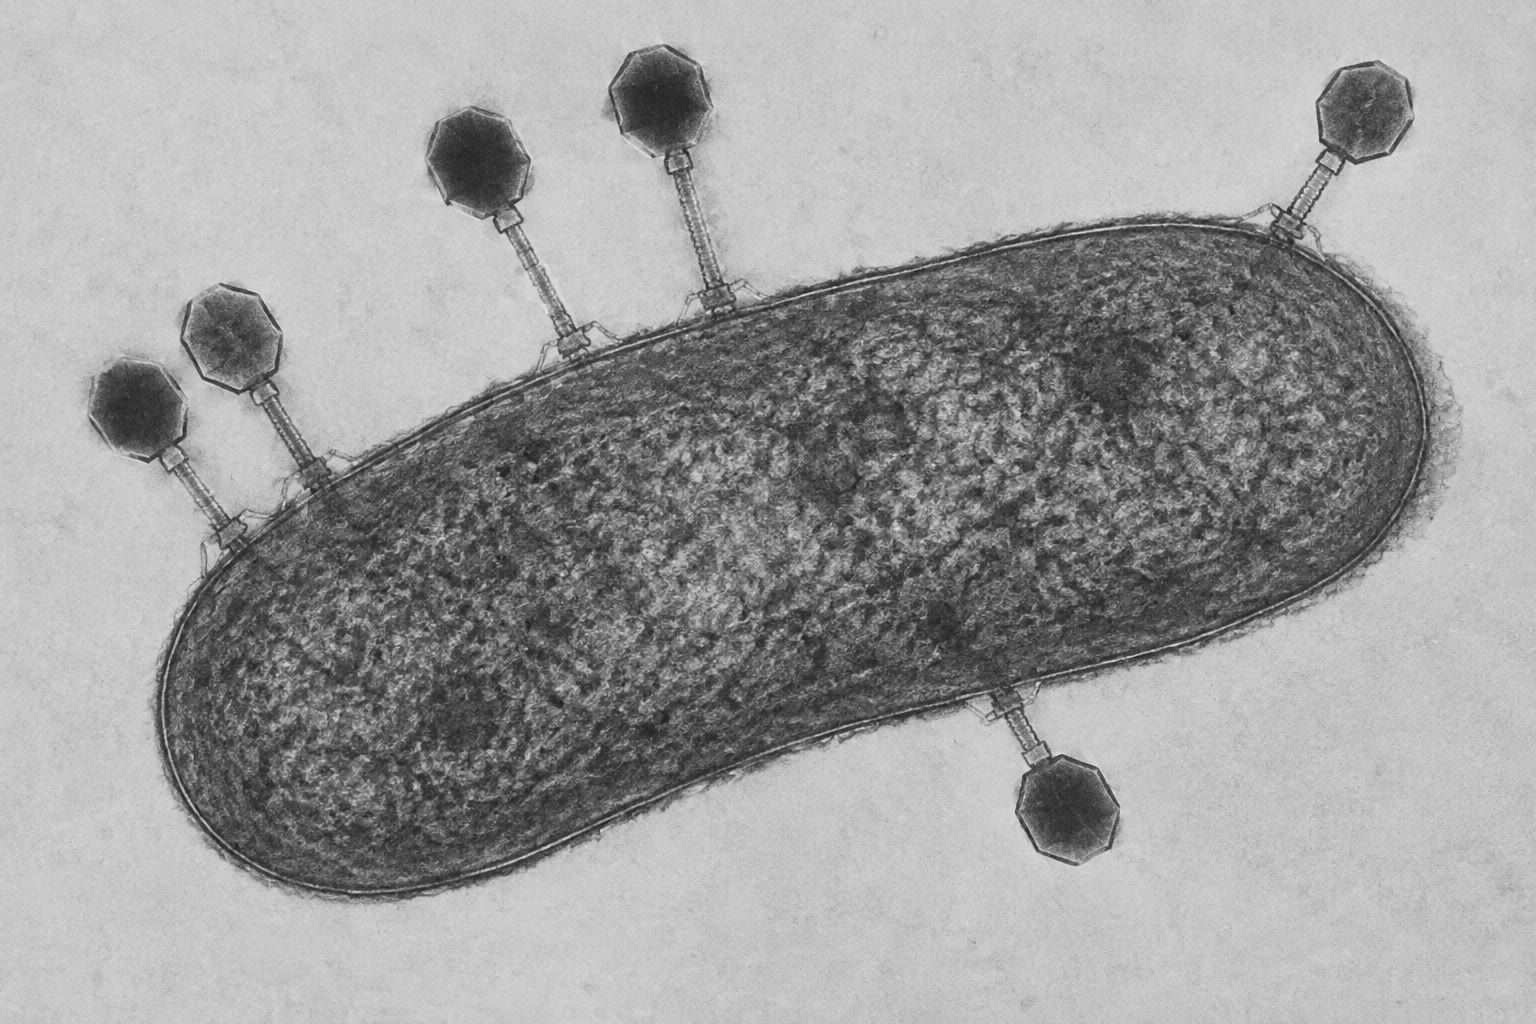
\includegraphics[width=0.5\linewidth]{images/book3/ai/b3-17-phage-on-bacterium.jpg}

{\small 附着在细菌上的噬菌体：多面体状的头部，
内装 \omterm{def:b1:nucleic-acids:chain}{DNA}，尾部用于将其注入。一个
\omterm{def:b1:cell-unit-of-life:cell}{细胞}可在半小时内释放一百个新噬菌体。}
\end{omfigure}

\begin{proposition}[噬菌体 $\lambda$ 的两种循环]\label{prop:b1:genomes:lambda}
\index{裂解循环}\index{溶原循环}
噬菌体 $\lambda$ 将其 \qty{48.5}{kb} 的 \omterm{def:b1:nucleic-acids:chain}{DNA}（见\cref{ch:b1:nucleic-acids}）
注入\emph{E. coli}，在其中环化。随后有两种去向：
在\emph{裂解循环}中，噬菌体\omterm{def:b1:genomes:gene}{基因}由宿主的
聚合酶转录，其 \omterm{def:b1:nucleic-acids:chain}{DNA} 被复制一百倍，\omterm{def:b1:genomes:virus}{衣壳}蛋白被合成
并组装，\omterm{def:b1:nucleic-acids:chain}{DNA} 装入其中，一种酶
溶解\omterm{def:b1:eukaryotic-cell:plantcell}{细胞壁}：\omterm{def:b1:cell-unit-of-life:cell}{细胞}破裂，释放出一百个噬菌体，
感染后四十分钟完成。在\emph{溶原循环}中，噬菌体 \omterm{def:b1:nucleic-acids:chain}{DNA}
插入宿主\omterm{def:b1:genomes:genome}{染色体}，并被其自身合成的阻遏蛋白
关闭：\emph{原噬菌体}随\omterm{def:b1:genomes:genome}{染色体}复制，
经历多代而不显现，直到宿主 \omterm{def:b1:nucleic-acids:chain}{DNA} 受损，
阻遏解除，裂解循环重新开始。这一选择是一个分子开关，
是最早被理解的分子开关之一（见\cref{ch:b1:expression-control}）。
\end{proposition}

\begin{omfigure}
\begin{tikzpicture}[font=\footnotesize, >=Stealth, line cap=round,
  st/.style={draw, thick, rounded corners=3pt, inner sep=3pt, align=center, fill=white}]
  \node[st, fill=omDef!12] (inj) at (0,0) {噬菌体 DNA 注入，\\ 环化};
  \node[st, fill=omThm!12] (rep) at (4.6,1.4) {复制、衣壳 \\ 蛋白、组装};
  \node[st, fill=omThm!12] (lys) at (9.2,1.4) {裂解：\qty{100}{} 个噬菌体 \\ 释放，\qty{40}{min}};
  \node[st, fill=omExo!12] (pro) at (4.6,-1.4) {整合为原噬菌体，\\ 被其阻遏蛋白关闭};
  \node[st, fill=omExo!12] (div) at (9.2,-1.4) {随宿主染色体 \\ 经多代复制};
  \draw[->, thick, omThm] (inj) -- (rep) node[pos=0.45, above left, omThm] {裂解};
  \draw[->, thick, omThm] (rep) -- (lys);
  \draw[->, thick, omExo!70!black] (inj) -- (pro) node[pos=0.4, below left, omExo!70!black] {溶原};
  \draw[->, thick, omExo!70!black] (pro) -- (div);
  \draw[->, thick, dashed, gray] (div.north) -- (lys.south) node[midway, right, align=left, font=\scriptsize] {诱导 \\ （宿主 DNA 受损）};
\end{tikzpicture}

{\small 噬菌体 $\lambda$：裂解循环（红色）或溶原循环（绿色），以及
将后者转变为前者的诱导过程。}
\end{omfigure}

\begin{example}[具有 RNA 基因组的病毒]\label{ex:b1:genomes:rna}
流感\omterm{def:b1:genomes:virus}{病毒}携带八段单链 \omterm{def:b1:nucleic-acids:chain}{RNA}，并自带
用于复制它们的聚合酶，因为\omterm{def:b1:cell-unit-of-life:cell}{细胞}中没有能复制 \omterm{def:b1:nucleic-acids:chain}{RNA} 的酶；
其聚合酶每 \num{10000} 个碱基出错一次，因此该\omterm{def:b1:genomes:virus}{病毒}
每个季节都会变化。逆转录\omterm{def:b1:genomes:virus}{病毒}（HIV）携带 \omterm{def:b1:nucleic-acids:chain}{RNA}，并带有一种
\emph{逆转录酶}，可将其复制为 \omterm{def:b1:nucleic-acids:chain}{DNA}，该 \omterm{def:b1:nucleic-acids:chain}{DNA} 插入
宿主\omterm{def:b1:genomes:genome}{染色体}，如同原噬菌体一样——形成持久感染。
其机制及免疫应答属于本科三年级分册的内容；
此处仅用于说明\omterm{def:b1:genomes:genome}{基因组}可能具有的范围。
\end{example}

\section{练习}

\begin{exercise}[$\star$]\label{exo:b1:genomes:1}
比较细菌与真核生物的\omterm{def:b1:genomes:genome}{基因组}：\omterm{def:b1:genomes:genome}{染色体}的数目与形态、
位置、\omterm{def:b1:body-plans-tissues:tissue}{组织}\omterm{def:b1:genomes:genome}{染色体}的\omterm{def:b1:proteins:peptide}{蛋白质}以及
\omterm{def:b1:genomes:gene}{基因}密度。
\end{exercise}

\begin{exercise}[$\star$]\label{exo:b1:genomes:2}
描述\omterm{def:b1:genomes:nucleosome}{核小体}，并给出\omterm{def:b1:genomes:nucleosome}{染色质}折叠各层级的
压缩倍数。
\end{exercise}

\begin{exercise}[$\star$]\label{exo:b1:genomes:3}
根据普查图，人类\omterm{def:b1:genomes:genome}{基因组}中编码\omterm{def:b1:proteins:peptide}{蛋白质}的部分占多大比例，
其中最大的一类是什么？
\end{exercise}

\begin{exercise}[$\star$]\label{exo:b1:genomes:4}
\omterm{def:b1:genomes:virus}{病毒}是什么？它在什么意义上不是活的？
\end{exercise}

\begin{exercise}[$\star\star$]\label{exo:b1:genomes:5}
计算 \emph{E. coli} \omterm{def:b1:genomes:genome}{染色体}的长度，以及若它是真核生物\omterm{def:b1:genomes:genome}{染色体}时所需的
以\omterm{def:b1:genomes:nucleosome}{核小体}为单位的圈数；
并说明细菌改用何种方式压缩它。
\end{exercise}

\begin{exercise}[$\star\star$]\label{exo:b1:genomes:6}
一个长 \qty{27}{kb} 的人类\omterm{def:b1:genomes:gene}{基因}，其\omterm{def:b1:genomes:gene}{外显子}总长 \qty{1.5}{kb}，
共八段。计算\omterm{def:b1:genomes:gene}{外显子}和\omterm{def:b1:genomes:gene}{内含子}的平均长度，
以及初级转录本中被舍弃部分所占的比例。
\end{exercise}

\begin{exercise}[$\star\star$]\label{exo:b1:genomes:7}
根据表格，计算 \emph{E. coli}、酵母、果蝇、人类和肺鱼的
每兆碱基的\omterm{def:b1:genomes:gene}{基因}数，并评论其变化趋势。
\end{exercise}

\begin{exercise}[$\star\star$]\label{exo:b1:genomes:8}
Alu 元件长 \qty{300}{bp}，共有一百万个拷贝。
Alu 元件占\omterm{def:b1:genomes:genome}{基因组}的比例是多少？若每个拷贝都经
逆转座（\omterm{def:b1:nucleic-acids:chain}{RNA} 被逆转录回 \omterm{def:b1:nucleic-acids:chain}{DNA} 并插入）产生，则每代需插入多少次，
才能在 6000 万年内产生一百万个拷贝，
按每代 \num{20} 年计？
\end{exercise}

\begin{exercise}[$\star\star$]\label{exo:b1:genomes:9}
解释\omterm{def:b1:eukaryotic-cell:mitochondrion}{线粒体}\omterm{def:b1:genomes:genome}{基因组}为何经母系遗传，
以及这对追溯祖源有何启示。
\end{exercise}

\begin{exercise}[$\star\star\star$]\label{exo:b1:genomes:10}
噬菌体 $\lambda$ 处于溶原状态时，每个宿主世代复制一次；处于裂解状态时，
可在 \qty{40}{min} 内产生一百个拷贝。在营养充足、每 \qty{20}{min}
分裂一次的培养物中，比较两种策略两小时内的情况；在不分裂的饥饿培养物中，
再次比较二者。
为何该开关会对宿主的
状况作出响应？
\end{exercise}

\begin{exercise}[$\star\star\star$]\label{exo:b1:genomes:11}
一个肺鱼\omterm{def:b1:cell-unit-of-life:cell}{细胞}携带 \qty{130}{Gb} 的 \omterm{def:b1:nucleic-acids:chain}{DNA}，计算其 \omterm{def:b1:nucleic-acids:chain}{DNA} 长度、每个\omterm{def:b1:cell-unit-of-life:cell}{细胞}中
\omterm{def:b1:genomes:nucleosome}{核小体}的数目与\omterm{def:b1:genomes:nucleosome}{组蛋白}的质量，并计算以人类复制叉速度（每个复制叉 \qty{50}{bp/s}）、
每 \qty{100}{kb} 设一个复制起点时，复制该\omterm{def:b1:genomes:genome}{基因组}所需的时间。
大\omterm{def:b1:genomes:genome}{基因组}给\omterm{def:b1:cell-unit-of-life:cell}{细胞}带来了何种代价？
\end{exercise}

\begin{exercise}[$\star\star\star$]\label{exo:b1:genomes:12}
“\omterm{def:b1:genomes:genome}{基因组}是一份记录，而不是设计。”请结合假\omterm{def:b1:genomes:gene}{基因}、转座元件、
\omterm{def:b1:genomes:gene}{基因}家族，以一段文字展开讨论，
并说明 C 值悖论。
\end{exercise}

\section{问题：六微米中的两米}

\begin{problem}[{周末问题——从螺旋到染色体测量人类细胞核：长度、
体积、核小体、组蛋白，以及各层级的堆积比，
最后得出中期染色体的
总压缩倍数}]
\label{pb:b1:genomes:1}
人类二倍体\omterm{def:b1:eukaryotic-cell:nucleus}{细胞核}为直径 \qty{6}{\micro m} 的球体，
含 46 条\omterm{def:b1:genomes:genome}{染色体}，共 $\num{6.4e9}$ 个\omterm{thm:b1:nucleic-acids:helix}{碱基对}；最大的\omterm{def:b1:genomes:genome}{染色体}携带 \qty{250}{Mb}，最小的为 \qty{50}{}。
取每对碱基长 \qty{0.34}{nm}，螺旋直径 \qty{2}{nm}，
每对碱基质量 \qty{650}{Da}，每个\omterm{def:b1:genomes:nucleosome}{核小体}含 \num{200} 对碱基，
\omterm{def:b1:genomes:nucleosome}{组蛋白}八聚体质量为 \qty{108}{kDa}，
每道尔顿取 $\qty{1.66e-24}{g}$。

\medskip
\noindent\textbf{第一部分——长度与体积。}
\begin{enumerate}
  \item 计算\omterm{def:b1:eukaryotic-cell:nucleus}{细胞核}中 \omterm{def:b1:nucleic-acids:chain}{DNA} 的总长度。
  \item 计算其中\omterm{thm:b1:nucleic-acids:helix}{双螺旋}的圈数。
  \item 计算最大与最小\omterm{def:b1:genomes:genome}{染色体}的
        \omterm{def:b1:nucleic-acids:chain}{DNA} 长度。
  \item 计算\omterm{def:b1:eukaryotic-cell:nucleus}{细胞核}的体积。
  \item 将 \omterm{def:b1:nucleic-acids:chain}{DNA} 视为圆柱体，计算其体积，
        以及它占\omterm{def:b1:eukaryotic-cell:nucleus}{细胞核}体积的比例。
  \item 计算\omterm{def:b1:eukaryotic-cell:nucleus}{细胞核}中 \omterm{def:b1:nucleic-acids:chain}{DNA} 的质量，以皮克计。
  \item \omterm{def:b1:eukaryotic-cell:nucleus}{细胞核}中约含 \qty{25}{pg} 的\omterm{def:b1:proteins:peptide}{蛋白质}。\omterm{def:b1:nucleic-acids:chain}{DNA} 占核质量的
        比例是多少？设水占\omterm{def:b1:eukaryotic-cell:nucleus}{细胞核}的 \qty{80}{\%}
        （密度为 \qty{1.1}{g/mL}）？
\end{enumerate}

\medskip
\noindent\textbf{第二部分——\omterm{def:b1:genomes:nucleosome}{核小体}。}
\begin{enumerate}[resume]
  \item 计算\omterm{def:b1:eukaryotic-cell:nucleus}{细胞核}中\omterm{def:b1:genomes:nucleosome}{核小体}的数目。
  \item 计算\omterm{def:b1:genomes:nucleosome}{组蛋白}的质量，并与
        \omterm{def:b1:nucleic-acids:chain}{DNA} 的质量进行比较。
  \item 一个\omterm{def:b1:genomes:nucleosome}{核小体}的 \qty{200}{} 对碱基在螺旋上跨越 \qty{68}{nm}，
        却占据长 \qty{11}{nm} 的珠子。计算“串珠”结构的
        压缩倍数。
  \item \qty{30}{nm} 纤维每 \qty{11}{nm} 的
        长度含六个\omterm{def:b1:genomes:nucleosome}{核小体}，计算其相对于裸 \omterm{def:b1:nucleic-acids:chain}{DNA} 的
        压缩倍数。
  \item 计算整个\omterm{def:b1:genomes:genome}{基因组}的 \qty{30}{nm} 纤维长度，
        并与\omterm{def:b1:eukaryotic-cell:nucleus}{细胞核}的直径进行比较。
  \item 每当 \omterm{def:b1:nucleic-acids:chain}{DNA} 被复制或转录时，每个\omterm{def:b1:genomes:nucleosome}{核小体}都须被拆开并重新组装。
        在 S 期（\qty{8}{h}）内有多少个\omterm{def:b1:genomes:nucleosome}{核小体}被重新组装？
        平均每秒有多少个？
\end{enumerate}

\medskip
\noindent\textbf{第三部分——环与\omterm{def:b1:genomes:genome}{染色体}。}
\begin{enumerate}[resume]
  \item \qty{30}{nm} 纤维的 \qty{75}{kb} 长的环从
        支架上悬挂下来。计算一个环中纤维的长度，
        以及\omterm{def:b1:genomes:genome}{基因组}中环的数目。
  \item 最大\omterm{def:b1:genomes:genome}{染色体}的一条中期染色单体长
        \qty{10}{\micro m}。计算从裸
        \omterm{def:b1:nucleic-acids:chain}{DNA} 到中期\omterm{def:b1:genomes:genome}{染色体}的压缩倍数。
  \item 将该染色单体视为
        直径为 \qty{0.7}{\micro m} 的圆柱体，计算其体积，
        以及其中 \omterm{def:b1:nucleic-acids:chain}{DNA} 所占的比例。
  \item 中期时的 46 条\omterm{def:b1:genomes:genome}{染色体}，每条都是
        密度相同的棒状体：计算它们的总体积，
        并与间期\omterm{def:b1:eukaryotic-cell:nucleus}{细胞核}进行比较。
  \item 解释为什么间期\omterm{def:b1:genomes:nucleosome}{染色质}不能像
        中期\omterm{def:b1:genomes:nucleosome}{染色质}那样紧密地折叠。
\end{enumerate}

\medskip
\noindent\textbf{第四部分——寻找\omterm{def:b1:genomes:gene}{基因}。}
\begin{enumerate}[resume]
  \item 一个\omterm{def:b1:proteins:peptide}{蛋白质}必须在\omterm{def:b1:genomes:genome}{基因组}中找一个 \qty{20}{bp} 的位点。
        若它每毫秒检测一个随机位点，搜索需要多长时间？
        这一结果说明位点
        是如何被找到的？
  \item \omterm{def:b1:genomes:genome}{基因组}中 \qty{20000}{} 个\omterm{def:b1:genomes:gene}{基因}平均长 \qty{27}{kb}。
        \omterm{def:b1:genomes:genome}{基因组}中位于\omterm{def:b1:genomes:gene}{基因}内部的部分占多大比例？
        编码部分占多大比例（每个\omterm{def:b1:genomes:gene}{基因}的\omterm{def:b1:genomes:gene}{外显子}总长为 \qty{1.5}{kb}）？
  \item 每条\omterm{def:b1:genomes:genome}{染色体}在\omterm{def:b1:eukaryotic-cell:nucleus}{细胞核}中各占一个区域。
        计算最大\omterm{def:b1:genomes:genome}{染色体}区域的体积，若区域体积与 \omterm{def:b1:nucleic-acids:chain}{DNA} 含量成正比，
        以及其内部 \omterm{def:b1:nucleic-acids:chain}{DNA} 的浓度（以
        \omterm{thm:b1:nucleic-acids:helix}{碱基对}每立方
        微米计）。
  \item 若一个肺鱼\omterm{def:b1:eukaryotic-cell:nucleus}{细胞核}的 \omterm{def:b1:nucleic-acids:chain}{DNA} 密度相同，
        \qty{260}{Gb}（二倍体）的 \omterm{def:b1:nucleic-acids:chain}{DNA} 对应的体积是多少？直径是多少？
  \item 计算\omterm{def:b1:cell-unit-of-life:cell}{细胞}在 S 期必须合成的\omterm{def:b1:genomes:nucleosome}{组蛋白}八聚体数目，
        以及它们所含的\omterm{def:b1:proteins:aminoacid}{氨基酸}数目（每个八聚体含 \qty{1000}{} 个残基）。
        并与\omterm{def:b1:cell-unit-of-life:cell}{细胞}一天内所合成的 \qty{3e9}{} 个
        \omterm{def:b1:proteins:peptide}{蛋白质}残基进行比较。
  \item 用两句话解释为什么细菌可以没有\omterm{def:b1:genomes:nucleosome}{核小体}，
        而真核生物不能。
  \item 给出结果：从\omterm{thm:b1:nucleic-acids:helix}{双螺旋}到中期\omterm{def:b1:genomes:genome}{染色体}的总压缩倍数，
        以及每一层级的压缩倍数。
\end{enumerate}
\end{problem}
